\subsection{Predicate Pushdown}\label{sec:match_optimize}
SeqStar can do further optimizations by analyzing the WHERE clause and push the predicates down to the star matching process.

The WHERE clause specifies extra constraints on the matching results in the form of predicates,
e.g., $u_2 > u_1$, $u_3 \le u_1$, etc.
And the Boolean operators AND, OR, NOT combine multiple predicates into a new one.
Semantically, the predicates connected by the AND operator can be checked separately.

\begin{figure}[ht]
  \centering
  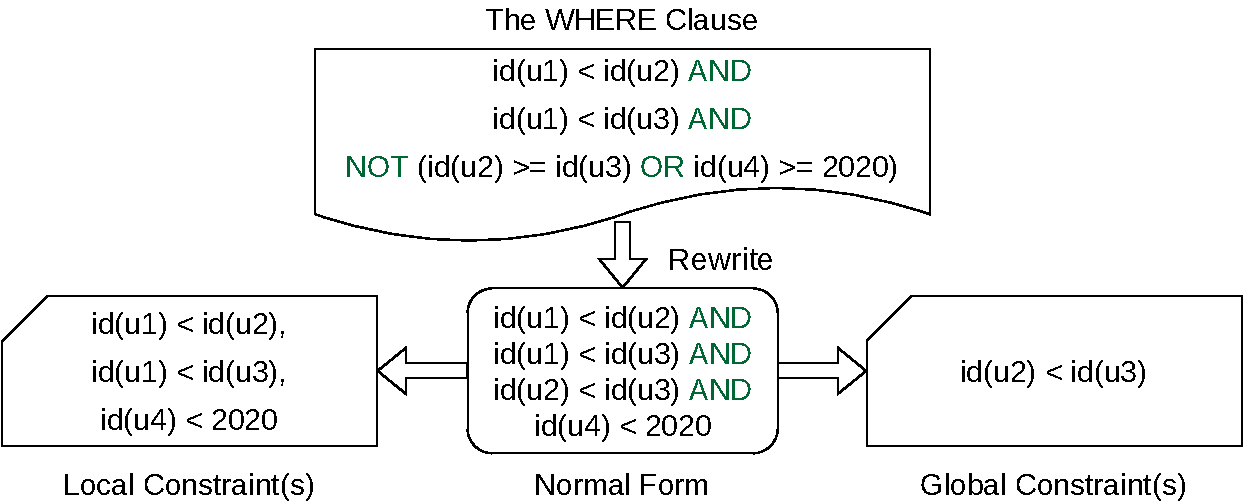
\includegraphics[width=.4\textwidth]{img/constraints.pdf}
  \caption{Constraint Analysis.}\label{img:constraints}
\end{figure}

SeqStar first applies De Morgan's law to rewrite the WHERE clause into AND-separated expressions as \emph{normal form}.
The expressions are then analyzed by Algorithm~\ref{alg:pushdown}.
SeqStar analyzes the syntax tree of each $expr$ and groups them into three categories:
(1) $\psi(u)$ is the predicate that has only one free variable $u$, e.g., $u_4 < 8$ (Figure~\ref{img:constraints});
(2) $\psi(u_1, u_2)$ has two free variables and edge exists between $u_1$, $u_2$, e.g., $u_2 > u_1$, $u_3 > u_1$;
(3) other predicates.
The predicates belong to (1) and (2) are bound to a star and we name it as \emph{local constraints}.
Local constraints can be applied during the star matching process to filter out unnecessary matchings.

\begin{algorithm}[ht]
  \caption{Predicate Pushdown}\label{alg:pushdown}
  \SetKwFunction{PredicatePushdown}{\textsc{PredicatePushdown}}
  \SetKwFunction{AddVertexConstraint}{\textsc{AddVertexConstraint}}
  \SetKwFunction{AddEdgeConstraint}{\textsc{AddEdgeConstraint}}
  \SetKwFunction{Edges}{\textsc{Edges}}
  \Fn{\PredicatePushdown{$exprs$, $p$}}{
    $globals \leftarrow \emptyset$\;
    \ForEach{$expr \in exprs$}{
      \Match{$expr$}{
        \Case{$\psi(u)$}{\AddVertexConstraint{$p$, $\psi(u)$}}
        \Case{$\psi(u_1, u_2)$}{
          \If{$(u_1, u_2) \in$ \Edges{$p$}}{\AddEdgeConstraint{$p$, $u_1$, $u_2$, $\psi(u_1, u_2)$}}
        }
        \Case{$e$}{$globals \leftarrow globals \cup \{e\}$\;}
      }
    }
    \Return{$globals$}
  }
\end{algorithm}

%% For example, in Figure~\ref{img:cypher_query}, there are three predicates concatenated by AND\@.
%% Formally, the constraint is a function $\psi: PG \rightarrow B$ with $PG$ the set of pattern graph and $B$ the set of Boolean values.
%% We will also use $\psi$ to denote abstract predicate for simplicity in this section:
%% $\psi(u)$ defines a constraint $\psi$ on vertex $u$, e.g., ``{id(u4) >= 2020}'' defines a vertex constraint on $u_4$ where the ID of the matching vertex of $u_4$ must great than or equal to $2020$;
%% and $\psi(u_1, u_2)$ defines a constraint on vertex $u_1$ and vertex $u_2$,
%% e.g., ``{id(u1) < id(u2)}'' defines a constraint on $u_1$ and $u_2$ that the ID of the matching of $u_1$ must be less than that of $u_2$.

%% Previous work usually ignore the constraint specification part of a graph matching query.
%% If someone wants to query a pattern with a specific searching condition,
%% she or he has to match the pattern graph first and then filter on the matching results,
%% which leaves a lot of room for improvement because the user provided searching conditions could filter out many unnecessary
%% partial results in an early phase.

%% However, it is still challenging to make use of the constraint provided by user's WHERE clause.
%% The pattern graph and the constraint are logically two different things,
%% we have to obtain enough information in order to use the constraint as early filter during the graph matching phase.
%% For example, the constraint in Figure~\ref{img:cypher_query} include all the vertices in the pattern graph,
%% only when the pattern graph is already matched could we got enough information to apply the constraint,
%% which makes the constraint filter nearly useless.

%% To address this problem, as shown in Figure~\ref{img:constraints},
%% we dive into the syntax tree of the graph matching query and decompose the searching condition into smaller parts which require only what we could got during the graph matching phase.
%% Specifically, we decompose the searching condition into three parts: \emph{vertex constraints}, \emph{edge constraints} and \emph{global constraint}.
%% A vertex constraint is a function $\psi(u)$ mapping vertex $u$ to Boolean values,
%% and an edge constraint sets a constraint on edge $(u_1, u_2)$ by a function $\psi(u_1, u_2)$.
%% For example, in Figure~\ref{img:pattern_graph} ``{id(u4) < 2020}'' sets a vertex constraint on $u_4$,
%% ``{id(u1) < id(u2)}'' and ``{id(u1) < id(u3)}'' are edge constraints,
%% while ``{id(u2) < id(u3)}'' is not because there is no edge between $u_2$ and $u_3$.
%% The \emph{vertex constraints} and \emph{edge constraints} are \emph{local constraints} that only require local information that can be obtained during the graph matching phase.
%% So they could then be pushed down to the data graph scanning phase to short-circuit useless matching results.
%% A global constraint $\psi(u_1, u_2, \dots)$ sets a constraint on a series of vertices $u_1, u_2, \dots$,
%% the information is insufficient during the data graph scanning phase.

%% \begin{algorithm}[ht]
%%   \caption{Constraint Rewriting}\label{alg:rewrite}
%%   \SetKwFunction{ConstraintRewrite}{\textsc{ConstraintRewrite}}
%%   \SetKwFunction{Simplify}{\textsc{Simplify}}
%%   \Input{$expr$: the abstract syntax tree of the WHERE clause}
%%   \Output{A set of simplified constraints connected by the AND ($\land$) operator}
%%   \Fn{\ConstraintRewrite{$expr$}}{
%%     \Match{$expr$}{
%%       \Case{$\lnot \lnot e$}{\Return{\ConstraintRewrite{$e$}}}
%%       \Case{$\lnot (e_1 \lor e_2)$}{
%%         \Return{\ConstraintRewrite{$\lnot e_1$} $\cup$ \ConstraintRewrite{$\lnot e_2$}}
%%       }
%%       \Case{$e_1 \land e_2$}{\Return{\ConstraintRewrite{$e_1$} $\cup$ \ConstraintRewrite{$e_2$}}}
%%       \Case{$e$}{\Return{$\{$ \Simplify{$e$} $\}$}}
%%     }
%%   }
%% \end{algorithm}

%% Logically, the AND ($\land$) operator create a new constraint $\psi = \psi_1 \land \psi_2$ by combining two constraints $\psi_1$ and $\psi_2$,
%% where $\psi_1$ and $\psi_2$ can be used to check the matching results independently because there is no side effects in constraints,
%% so we could safely split $\psi$ into $\psi_1$ and $\psi_2$.
%% Because local constraints are the earliest constraint filters, we should extract as much as possible.
%% In order to make the constraint filters more efficient and extract more local constraints:
%% Firstly, we optimize the AST by classic methods such as compile-time calculation,
%% handle special cases such as ``{WHERE false}''.
%% Then, we apply Algorithm~\ref{alg:rewrite} to analyze the syntax tree and rewrite it into \emph{normal form},
%% where a normal form is a list of simplified constraints connected by the AND operator.
%% In fact, the constraints are mostly specified by binary operators such as ``$\le$'', ``$\ne$'',
%% hence many constraints are naturally local constraints.
%% And the De Morgan's law enables us to convert the OR ($\lor$) operator into AND ($\land$):
%% \begin{equation}
%%   \lnot (\psi_1 \lor \psi_2) = \lnot \psi_1 \land \lnot \psi_2
%% \end{equation}
%% So Algorithm~\ref{alg:rewrite} will always keep the semantics of the original user provided constraint.
%% For example, the third predicate of the AND operator in Figure~\ref{img:cypher_query} would be rewritten to
%% \begin{verbatim}
%%   id(u2) < id(u3) AND id(u4) < 2020
%% \end{verbatim}
%% by applying De Morgan's law.
%% And the WHERE clause of Figure~\ref{img:cypher_query} would be rewritten to the normal form:
%% \begin{verbatim}
%%   WHERE id(u1) < id(u2) AND id(u1) < id(u3)
%%   AND id(u2) < id(u3) AND id(u4) < 2020
%% \end{verbatim}

%% The normal form is then used to extract useful information to be pushed down to the pattern graph as in Algorithm~\ref{alg:push_down}.
%% For each constraint in the normal form, we check if it is local constraint and then push it down to the corresponding vertex or edge.
%% After that, We could then decompose it into stars.
%% Our framework contains a JIT compiler that is able to emit callable closures based on the AST,
%% and the local constraints can then be used to serve as early filters in the data graph scanning process to short-circuit unnecessary matchings as soon as possible.
%% \subsubsection{Star Isomorphism}
%% Consider Figure~\ref{img:star_decomposition}, we generate three stars from the original pattern,
%% and these stars are isomorphic with each other.
%% Therefore the matching results of these stars are always the same,
%% there is no need to match these stars again and again.
%% Though the general graph isomorphism problem is NP complete,
%% the isomorphism of stars are easier to check.
%% We say that our stars in Figure~\ref{img:star_decomposition} belong to the same \textsc{Characteristic} equivalence class,
%% where \text{Characteristic} is a structure that stores the root and neighbors in a predefined order.
%% By grouping isomorphic stars into the same \textsc{Characteristic} equivalence class,
%% we could avoid unnecessary computation.
